
This sections will provide new tools and ideas to analyze games and to do that, the same strategy of the previous section will be followed. Initially, the reader is presented with an intuitive idea and preliminary formulation of the problem. The first part contains many examples and its intent is to provide the reader enough to use the more mathematical heavy part to in fact gain advantage in any game played.

Now that enough is known about numbers, it is possible to work with non-numbers. The only known non-numbers at this point are the switches. But is knowing what they are enough to playing them? The game simpler cashing cheques will tell.

In this game there is a table with purple cheques. Each cheque has two numbers written on top, and, in each player's turn they will either pay one coin or cash a cheque that will grant him a number of coins equal to the correspondent associated integer. What is the best move for Left?

\begin{center}
\begin{tikzpicture}
	\node[draw] (title) at (0,1.5) {\textbf{Simpler Cashing Cheques}};
	\begin{scope} [every node/.style={style=circle, draw, fill=purple2}]
		\node at (-2,0) {8 $|$ 4};
		\node at (0,0) {5 $|$ 5};
		\node at (2,0) {1 $|$ 13};
	\end{scope}
\end{tikzpicture}
\end{center}

Definitely the move is not paying, as Left can earn money in his turn. A good thing to grasp from this example is that you should never play in a number, paying a coin in this case, if there are non-numbers, cashing a purple cheque in this case. Should Left cash 8, 5 or 1? 1, of course. The reader is encouraged to play as Left and trying to find the best possible outcome, but the answer is playing the hottest switch. Although the game above is not a switch, it is a sum of switches, and, because of that can benefit of the simplified notation discussed earlier.

\begin{align*}
	G =& \left(\frac{8-4}{2} \pm \frac{8+4}{2}\right) + \left(\frac{5-5}{2} \pm \frac{5+5}{2}\right) + \left(\frac{1-13}{2} \pm \frac{1+13}{2}\right) \\
	  =& (2 \pm 6) + (0 \pm 5) + (-6 \pm 7)\\
	  =& -4 \pm 7 \pm 6 \pm 5
\end{align*}

If you analyze the result above, it becomes clear that Left must play on the rightmost component as, although it will not provide many coins, it will prevent right from cashing a huge amount. It is very possible to build scenarios where a player would even pay for cashing a cheque if that prevented the opponent from getting rich. Now that playing a simpler cashing cheques became easy, a more challenging task will rise. How to play Domineering well?

Adding a number with a temperature in a simplified position, like the expression above, should be acceptable by anyone following up to this point. Following, in the other hand, numbers will be added together with non-numbers just like number are added together and this might cause confusion. However, understanding that this sum is possible and intuitive is simple.

Playing a sum of games is just like playing a game with a set of independent rulesets and components. \begin{center}
	\begin{tikzpicture}
		\node at (-0.5,0.1) {G =};
		\draw[] (0,0) rectangle ++(0.3,0.3);
		\draw[] (0.3,0) rectangle ++(0.3,0.3);
		\draw[] (0.6,0) rectangle ++(0.3,0.3);
		\node at (1.2,0.1) {$+$};
		\node[style=circle, draw, fill=purple2] at (2.1,0.1) {8 $|$ 4};
		\node at (3.1,0.1) {$+$};
		\draw[color=blue, ultra thick] (3.4, -0.1) -- (3.4, 0.5);
		\node[] at(3.6, -0.1) {,};
		\end{tikzpicture}
\end{center}
for example, is a game where each player makes a move\footnote{There are other ways of playing G that will not be discussed} in any of the components and loses if cannot make a move. In other words, \Gm{} is a game like every other, except for the more complex ruleset.

The result of this sum is obvious if all components are also numbers or switches. In the case of playing numbers and general non-numbers, sensible players will always play in non-numbers first. With this in mind other facts become clear. The first is that the temperature of a non-number added to a number is unaltered.

The second is that such a sum is actually a sum of non-numbers, added together with a number after they cool out. The sum of general non-numbers is thoroughly discussed in the remaining of the chapter, however, it worth noticing what the goal of this discussion is.

By the end of this section it will be thought how to convert any game in a 2D graphic composed of two trajectories that collapse to one line at some point, whose axis are number and cooling factor. The purpose of all this is that if the ending point falls in the positive side, Left gets an advantage, and if it falls in the positive, right does.

To build this graphic one is required to traverse the game tree, so the effort may seem fruitless as the game tree itself provides the winning strategy by itself. However, in cases where the game tree resulting from the sum of games is too large or expensive for a computer to run, there is a good strategy to playing this sum without knowing the complete game tree. In order to build the thermograph and play the \defi{thermostrat}\footnote{This text will not present the thermostrat} correctly, there are a lot of minor concepts not discussed yet.

Other than the bias, playing a game like Domineering well involves the concepts of \defi{Left/Right stops}, \defi{toenail}, \defi{ambient temperature}, \defi{freezing point}, \defi{cooling}, \defi{heating} and a few others. To put all that together and provide a clear visualization of the best strategy, the thermograph.

\begin{center}
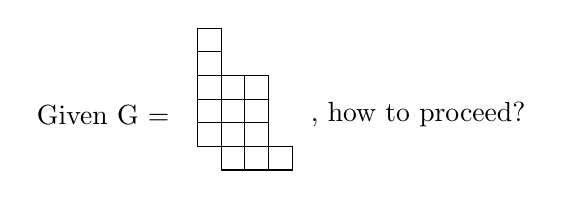
\begin{tikzpicture}
	\node at (-1.5,0.1) {Given G =};
	\draw[] (0,-0.6) rectangle ++(0.3,0.3);
	\draw[] (0.3,-0.6) rectangle ++(0.3,0.3);
	\draw[] (0.6,-0.6) rectangle ++(0.3,0.3);
	\draw[] (-0.3,-0.3) rectangle ++(0.3,0.3);
	\draw[] (0,-0.3) rectangle ++(0.3,0.3);
	\draw[] (0.3,-0.3) rectangle ++(0.3,0.3);
	\draw[] (-0.3,0) rectangle ++(0.3,0.3);
	\draw[] (0,0) rectangle ++(0.3,0.3);
	\draw[] (0.3,0) rectangle ++(0.3,0.3);
	\draw[] (-0.3,0.3) rectangle ++(0.3,0.3);
	\draw[] (0,0.3) rectangle ++(0.3,0.3);
	\draw[] (0.3,0.3) rectangle ++(0.3,0.3);
	\draw[] (-0.3,0.6) rectangle ++(0.3,0.3);
	\draw[] (-0.3,0.9) rectangle ++(0.3,0.3);
	\node at (2.5,0.1) {, how to proceed?};
\end{tikzpicture}
\end{center}

\begin{center}
	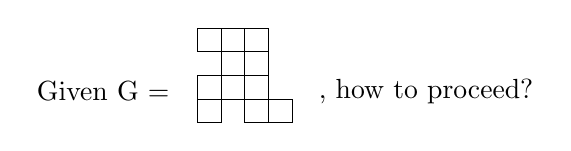
\begin{tikzpicture}
		\node at (-1.2,0.1) {Given G =};...
		\draw[] (0.6,-0.3) rectangle ++(0.3,0.3);
		\draw[] (0.9,-0.3) rectangle ++(0.3,0.3);
		\draw[] (0,-0.3) rectangle ++(0.3,0.3);
		\draw[] (0,0) rectangle ++(0.3,0.3);
		\draw[] (0.3,0) rectangle ++(0.3,0.3);
		\draw[] (0.6,0) rectangle ++(0.3,0.3);
		\draw[] (0.3,0.3) rectangle ++(0.3,0.3);
		\draw[] (0.6,0.3) rectangle ++(0.3,0.3);
		\draw[] (0,0.6) rectangle ++(0.3,0.3);
		\draw[] (0.3,0.6) rectangle ++(0.3,0.3);
		\draw[] (0.6,0.6) rectangle ++(0.3,0.3);
		\node at (2.9,0.1) {, how to proceed?};
	\end{tikzpicture}
\end{center}

G is definitely not a switch nor a sum of switches. It is possible to say the temperature in G is going to stay high for quite some time, because hotness is a term used to define the importance of the next move. A good place to start is writing out the game tree and building a temperature graphic of how it builds up from simpler positions until the more complicated ones.

To decrease the confusion that builds up in complicated positions, there is the idea of a cooling factor. The non-number \Gm{} cooled by $t$ degrees is represented by \Gm{_t} and is defined by:
\begin{center}
	\Gm{_t} = \gam{\Gm{^L_t} - t}{\Gm{^R_t} + t} $\forall t \leq t'$\\
	\Gm{_t} = x $\forall t > t'$\\
	Given $t'$ is the smallest cooling factor such\\
	that \Gm{_{t'}} is infinitesimally close to a number $x$,
\end{center}

The temperature $t(G)$ is equal to $t'$. Now that both axes are defined, some examples of thermographs:

\begin{tikzpicture}
	\begin{axis}
		[
		title = \Gm{=} \gam{3}{1},
		xmin=0.5,xmax=3.5, x dir=reverse, xtick={0, 1, 2, 3},
		ymax=3, ytick={0, 0.5, 1},
		axis x line*=none, axis y line*=none,
		axis line style={draw=none},
		y label style={rotate=-90,at={(current axis.north west)}, right=5mm},
		ylabel = \textbf{t}
		]
		\addplot[black] coordinates {
		(0.5,0)(3.5,0)
		};
		\addplot[black, very thick] coordinates {
		(0.9,-0.1)(2,1)
		};
		\addplot[black, very thick] coordinates {
		(3.1,-0.1)(2,1)
		};
		\addplot[black,-{Latex[length=3mm]}, very thick] coordinates {
		(2,1)(2,2)
	};
	\end{axis}
	\begin{axis}
	[
	at={(0.5\linewidth,0)},
	title = \Gm{=} \gam{0}{{-}4},
	xmin=-4.5,xmax=0.5, x dir=reverse, xtick={-4, -2, 0},
	ymax=3, ytick={0, 1, 2},
	axis x line*=none, axis y line*=none,
	axis line style={draw=none},
	y label style={rotate=-90,at={(current axis.north west)}, right=5mm},
	ylabel = \textbf{t}
	]
	\addplot[black] coordinates {
		(0.5,0)(-4.5,0)
	};
	\addplot[black, very thick] coordinates {
		(-0.1,-0.1)(-2,2)
	};
	\addplot[black, very thick] coordinates {
		(-4.1,-0.1)(-2,2)
	};
	\addplot[black,-{Latex[length=3mm]}, very thick] coordinates {
		(-2,2)(-2,2.5)
	};
	\end{axis}
	\begin{axis}
	[
	at={(0,-330)},
	title = \Gm{=} \gam{0}{0},
	xmin=-0.5,xmax=0.5, x dir=reverse, xtick={0},
	ymax=2, ytick={0, 1},
	axis x line*=none, axis y line*=none,
	axis line style={draw=none},
	y label style={rotate=-90,at={(current axis.north west)}, right=5mm},
	ylabel = \textbf{t}
	]
	\addplot[black] coordinates {
		(-0.5,0)(0.5,0)
	};
	\addplot[black, very thick] coordinates {
		(-0.1,-0.1)(0,0)
	};
	\addplot[black, very thick] coordinates {
		(0.1,-0.1)(0,0)
	};
	\addplot[black,-{Latex[length=3mm]}, very thick] coordinates {
		(0,0)(0,1.5)
	};
	\end{axis}
	\begin{axis}
	[
	at={(0.5\linewidth,-330)},
	title = \Gm{=} \gam{0}{\gam{0}{0}},
	xmin=-0.5,xmax=0.5, x dir=reverse, xtick={0},
	ymax=2, ytick={0, 1},
	axis x line*=none, axis y line*=none,
	axis line style={draw=none},
	y label style={rotate=-90,at={(current axis.north west)}, right=5mm},
	ylabel = \textbf{t}
	]
	\addplot[black] coordinates {
		(-0.5,0)(0.5,0)
	};
	\addplot[black, very thick] coordinates {
		(0,-0.1)(0,0)
	};
	\addplot[black, very thick] coordinates {
		(0.1,-0.1)(0,0)
	};
	\addplot[black,-{Latex[length=3mm]}, very thick] coordinates {
		(0,0)(0,1.5)
	};
	\end{axis}
\end{tikzpicture}


Some characteristics might be immediately apparent. The first is that the x-axis is reversed. The reason for that is to keep Right's movements to the right and Left's to the left. The second characteristic may be that all the thermographs end with a vertical \defi{mast}. The mast begins at $t'$ and indicates that \Gm{} is a number from that point forward. The last one is that the graphic continues past the $y=0$ line. It is worth noticing that the difference between the last two thermographs is below the $y=0$ line.

Toenails, the segments below the $y=0$ line, are important and may seem different, but they are actually simple extensions of the graphic. The reason for the last two toenails to be different is that cooling is applied to all the Left and Right alternatives, but in opposite directions. It is important to remember \hbox{\Gm{_t} = \gam{\Gm{^L_t} - t}{\Gm{^R_t} + t}}, because it explains the difference. Both Left's and the first Right's toenail came from cooling 0, but the second Right's toenail came from cooling \gam{0}{0}.

The next example, the second of non-switch hot games, shows how cooling $L$ and $R$ alternatives work.\\

\begin{figure}[H]
\begin{center}
	\scalebox{0.8}{
\begin{tikzpicture}
	\node[] at (2.2, 6.6) {\textbf{Freezing point}};
	\node[scale=0.5, circle, draw, fill=black] at (4.2, 6.6) {};
	\begin{axis}
		[
		title = \Gm{=}\gam{\gam{3}{1}}{\gam{0}{{-}4}},
		xmin=-4.5,xmax=3.5, x dir=reverse, xtick={-2, -4, 0, 1, 2, 3},
		ymax=2.5, ytick={0, 0.5, 1, 2},
		axis x line*=none, axis y line*=none,
		axis line style={draw=none},
		y label style={rotate=-90,at={(current axis.north west)}, right=5mm},
		ylabel = \textbf{t},
		scale=1.4
		]
		
		\addplot[black] coordinates {
			(-4.5,0)(3.5,0)
		};
		\addplot[ultra thick] coordinates {
			(0.9,-0.1)(2,1)
		};
		\addplot[black] coordinates {
			(3.1,-0.1)(2,1)
		};
		\addplot[-{Latex[length=3mm]}, ultra thick] coordinates {
			(2,1)(2,2.5)
		};
		\addplot[ultra thick] coordinates {
			(0.1,-0.1)(-2,2)
		};
		\addplot[] coordinates {
			(-4.1,-0.1)(-2,2)
		};
		\addplot[-{Latex[length=3mm]}, ultra thick] coordinates {
			(-2,2)(-2,2.5)
		};
		\addplot[black, dashed, ultra thick] coordinates {
			(1,-0.1)(1,1)
		};
		\addplot[black, dashed, ultra thick] coordinates {
			(0,-0.1)(0,2)
		};
		\addplot[black, dashed, ultra thick] coordinates {
			(1,1)(0,2)
		};
		\addplot[black, dashed] coordinates {
			(0,2)(-1,3)
		};
		\addplot[black, dashed] coordinates {
			(0,2)(0.5,2.5)
		};
		\addplot[black, dashed, ultra thick, -{Latex[length=3mm]}] coordinates {
			(0,2)(0,2.5)
		};
	\end{axis}
\end{tikzpicture}}
\end{center}
\caption{The dissection of a thermograph}
\end{figure}



In the example above, the thick dashed thermograph is the thermograph of G. The light dashed segments are illustrative extensions of the cooling of L and R. The bold lines were used to show what part of L and R are taken into consideration: Right's slant is used to build Left's slant and vice-versa. The reason for this is that after either player makes a move, it will be the opponent's turn to move, and, this way, the opposing slant is the important one.

It is also worth mentioning that a freezing point will always be reached after an equal amount of move by each player. In the example above, the freezing point is the same as the junction point where the right slant bends, but that is not always the case. Before visiting Siegel's formulation of the problem, one that brings good notation and formalism, an example of a real scenario is due. In a fun game each player has more than one option for their moves and that has not been addressed yet.

What is the thermograph of the game \Gm{=}
	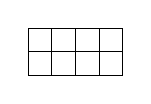
\begin{tikzpicture}
		\draw[] (0.6,-0.6) rectangle ++(0.3,0.3);
		\draw[] (0.3,-0.6) rectangle ++(0.3,0.3);
		\draw[] (0.9,-0.6) rectangle ++(0.3,0.3);
		\draw[] (0,-0.6) rectangle ++(0.3,0.3);
		\draw[] (0,-0.3) rectangle ++(0.3,0.3);
		\draw[] (0.3,-0.3) rectangle ++(0.3,0.3);
		\draw[] (0.6,-0.3) rectangle ++(0.3,0.3);
		\draw[] (0.9,-0.3) rectangle ++(0.3,0.3);
	\end{tikzpicture} ? 

\begin{figure} [!ht]
\begin{center}
\begin{tikzpicture}
	[
	sibling distance=150pt,
	level distance=100pt,
	level 1/.style={sibling distance=4cm},
	level 2/.style={sibling distance=1.7cm},
	every node/.style = {
	},
	every child/.style = {
		ultra thick
	}
	]

\node[draw] (title) at (0, 1) {Game Tree};

\node {
	\begin{tikzpicture}
		\draw[] (0.6,-0.6) rectangle ++(0.3,0.3);
		\draw[] (0.3,-0.6) rectangle ++(0.3,0.3);
		\draw[] (0.9,-0.6) rectangle ++(0.3,0.3);
		\draw[] (0,-0.6) rectangle ++(0.3,0.3);
		\draw[] (0,-0.3) rectangle ++(0.3,0.3);
		\draw[] (0.3,-0.3) rectangle ++(0.3,0.3);
		\draw[] (0.6,-0.3) rectangle ++(0.3,0.3);
		\draw[] (0.9,-0.3) rectangle ++(0.3,0.3);
	\end{tikzpicture}}
child[blue, level distance=80pt] {node[black] {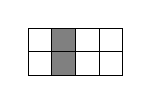
\begin{tikzpicture}
			\draw[] (0.6,-0.6) rectangle ++(0.3,0.3);
			\draw[fill=gray] (0.3,-0.6) rectangle ++(0.3,0.3);
			\draw[] (0.9,-0.6) rectangle ++(0.3,0.3);
			\draw[] (0,-0.6) rectangle ++(0.3,0.3);
			\draw[] (0,-0.3) rectangle ++(0.3,0.3);
			\draw[fill=gray] (0.3,-0.3) rectangle ++(0.3,0.3);
			\draw[] (0.6,-0.3) rectangle ++(0.3,0.3);
			\draw[] (0.9,-0.3) rectangle ++(0.3,0.3);
	\end{tikzpicture}}
	child[blue] {node[black] {\gam{1}{}}}
	child[blue] {node[black] {\gam{1}{{-}1}}}
	child[red, dashed] {node[black] {\gam{{-}1}{1}}}
}
child[blue] {node[black] {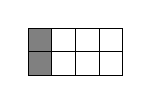
\begin{tikzpicture}
			\draw[] (0.6,-0.6) rectangle ++(0.3,0.3);
			\draw[] (0.3,-0.6) rectangle ++(0.3,0.3);
			\draw[] (0.9,-0.6) rectangle ++(0.3,0.3);
			\draw[fill=gray] (0,-0.6) rectangle ++(0.3,0.3);
			\draw[fill=gray] (0,-0.3) rectangle ++(0.3,0.3);
			\draw[] (0.3,-0.3) rectangle ++(0.3,0.3);
			\draw[] (0.6,-0.3) rectangle ++(0.3,0.3);
			\draw[] (0.9,-0.3) rectangle ++(0.3,0.3);
	\end{tikzpicture}}
	child[blue] {node[black] {\gam{1}{}}}
	child[blue] {node[black] {\gam{1}{{-}1}}}
	child[red, dashed] {node[black] {\gam{{-}1}{0,1}}}
}
child[red, dashed, level distance=80pt] {node[black, solid] { 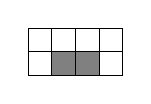
\begin{tikzpicture}
			\draw[fill=gray] (0.6,-0.6) rectangle ++(0.3,0.3);
			\draw[fill=gray] (0.3,-0.6) rectangle ++(0.3,0.3);
			\draw[] (0.9,-0.6) rectangle ++(0.3,0.3);
			\draw[] (0,-0.6) rectangle ++(0.3,0.3);
			\draw[] (0,-0.3) rectangle ++(0.3,0.3);
			\draw[] (0.3,-0.3) rectangle ++(0.3,0.3);
			\draw[] (0.6,-0.3) rectangle ++(0.3,0.3);
			\draw[] (0.9,-0.3) rectangle ++(0.3,0.3);
	\end{tikzpicture}}
	child[blue, solid] {node[black] {\gam{{-}1}{0, 1}}}
	child[red] {node[black] {\gam{1}{}}}
	child[red] {node[black] {\gam{0}{0}}}
}
child[red, dashed] {
	node[black, solid] { 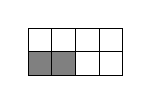
\begin{tikzpicture}
	\draw[] (0.6,-0.6) rectangle ++(0.3,0.3);
	\draw[fill=gray] (0.3,-0.6) rectangle ++(0.3,0.3);
	\draw[] (0.9,-0.6) rectangle ++(0.3,0.3);
	\draw[fill=gray] (0,-0.6) rectangle ++(0.3,0.3);
	\draw[] (0,-0.3) rectangle ++(0.3,0.3);
	\draw[] (0.3,-0.3) rectangle ++(0.3,0.3);
	\draw[] (0.6,-0.3) rectangle ++(0.3,0.3);
	\draw[] (0.9,-0.3) rectangle ++(0.3,0.3);
	\end{tikzpicture}}
		child[blue, solid] {node[black] {\gam{{-}1}{1}}}
		child[blue, solid] {node[black] {\gam{{-}1}{0,1}}}
		child[red] {node[black] {\gam{}{{-}1}}}
	}
;

\end{tikzpicture}
\end{center}
\end{figure}

\hspace{-1cm}
\begin{tikzpicture}
\begin{axis}
	[
		title = \gam{\gam{1}{{-}1},2}{0},
		xmin=-1.5,xmax=2.5, x dir=reverse, xtick={-1,0, 1, 2},
		ymax=2, ytick={0, 1, 1},
		scale=0.5,
		style thermograph
	]
	\addplot[] coordinates {(3.5,0)(-1.5,0)};
	\addplot[-{Latex[length=3mm]}] coordinates { (2,-0.1)(2,1.5)};
	\addplot[-{Latex[length=3mm]}] coordinates { (0,-0.1)(0,1.5)};
	\addplot[ultra thick] coordinates { (-0.1,-0.1)(1,1)};
	\addplot[ultra thick] coordinates { (2.1,-0.1)(1,1)};
	\addplot[-{Latex[length=3mm]}, ultra thick] coordinates { (1,1)(1,1.9)};
	\addplot[] coordinates {(1.1,-0.1)(0,1)};
	\addplot[red, densely dashed] coordinates {(-1.1,-0.1)(0,1)};
\end{axis}
\begin{axis}
	[
	title = \gam{2,\gam{1}{{-}1}}{{-}\frac{1}{2}},
	xmin=-1.5,xmax=2.5, x dir=reverse, xtick={-0.5, 1.25,2},
	ymax=2.3, ytick={0, 1.25},
	scale=0.5,
	at={(4cm,0)},
	style thermograph
	]
	\addplot[] coordinates {(2.5,0)(-1.5,0)};
	\addplot[-{Latex[length=3mm]}] coordinates { (2,-0.1)(2,1.5)};
	\addplot[-{Latex[length=3mm]}] coordinates { (-0.5,-0.1)(-0.5,1.5)};
	\addplot[ultra thick] coordinates { (-0.6,-0.1)(0.75,1.25)};
	\addplot[ultra thick] coordinates { (2.1,-0.1)(0.75,1.25)};
	\addplot[-{Latex[length=3mm]}, ultra thick] coordinates { (0.75,1.25)(0.75,2.2)};
	\addplot[] coordinates {(1.1,-0.1)(0,1)};
	\addplot[red, densely dashed] coordinates {(-1.1,-0.1)(0,1)};
	\addplot[-{Latex[length=3mm]}] coordinates { (0,1)(0,1.5)};
\end{axis}
\node[] at (9.3,2) {\gam{{-}\frac{1}{2}}{2, \gam{0}{0}}};
\node[] at (9.3,1.5) {$=0$};
\begin{axis}
	[
	title = \gam{{-}\frac{1}{2}, 0}{{-}2},
	xmin=-2.5,xmax=0.5, x dir=reverse, xtick={-2,-1,0},
	ymax=2.5, ytick={0, 1, 1.75},
	scale=0.5,
	at={(12cm,0)},
	style thermograph
	]
	\addplot[] coordinates {(-3.5,0)(1.5,0)};
	\addplot[-{Latex[length=3mm]}] coordinates { (0,-0.1)(0,1.5)};
	\addplot[-{Latex[length=3mm]}] coordinates { (-0.5,-0.1)(-0.5,1.5)};
	\addplot[-{Latex[length=3mm]}] coordinates { (-2,-0.1)(-2,1.5)};
	\addplot[ultra thick] coordinates {(0.1,-0.1)(-1,1)};
	\addplot[ultra thick] coordinates { (-2.1,-0.1)(-1,1)};
	\addplot[-{Latex[length=3mm]}, ultra thick] coordinates { (-1,1)(-1,1.75)};
\end{axis}
\end{tikzpicture}

\hspace{-2.3cm}
\begin{tikzpicture}
\begin{axis}
	[
	title = \Gm{},
	xmin=-2.5,xmax=2.5, x dir=reverse, xtick={-2,-1,0,1,2},
	ymax=2.5, ytick={0, 1, 1.75},
	scale=1,
	at={(0,-7.5cm)},
	style thermograph
	]
	\addplot[] coordinates {(-2.5,0)(2.5,0)};
	\addplot[] coordinates {(0.1,-0.1)(-1,1)};
	\addplot[] coordinates { (-2.1,-0.1)(-1,1)};
	\addplot[] coordinates { (2.1,-0.1)(0.75,1.25)};
	\addplot[] coordinates { (2.1,-0.1)(1,1)};
	\addplot[] coordinates { (1,1)(-0.1,-0.1)};
	\addplot[] coordinates { (0.75,1.25)(-0.6,-0.1)};
	\addplot[-{Latex[length=3mm]}] coordinates { (-1,1)(-1,1.75)};
	\addplot[-{Latex[length=3mm]}] coordinates { (0,-0.1)(0,1.5)};
	\addplot[-{Latex[length=3mm]}] coordinates { (0.75,1.25)(0.75,2.3)};
	\addplot[-{Latex[length=3mm]}] coordinates { (1,1)(1,2.3)};
\end{axis}
\node[] at (7.5,-5) {$\underset{\text{Removing  dominated moves}}{\Rightarrow}$};
\begin{axis}
	[
	title = \Gm{},
	xmin=-0.5,xmax=2.5, x dir=reverse, xtick={2,1,0},
	ymax=2.5, ytick={0, 1, 1.75},
	scale=1,
	at={(0.5*\linewidth + 2cm,-7.5cm)},
	style thermograph
	]
	\addplot[] coordinates {(-2.5,0)(2.5,0)};
	\addplot[] coordinates { (2.1,-0.1)(1,1)};
	\addplot[] coordinates { (1,1)(-0.1,-0.1)};
	\addplot[] coordinates { (-0.1,-0.1)(0,0)};
	\addplot[-{Latex[length=3mm]}] coordinates { (0,-0.1)(0,1.5)};
	\addplot[-{Latex[length=3mm]}] coordinates { (1,1)(1,2.3)};
\end{axis}
\end{tikzpicture}
\begin{center}
\begin{tikzpicture}
\begin{axis}
	[
	title = \Gm{},
	xmin=-1.5,xmax=1.5, x dir=reverse, xtick={1,0,-1},
	ymax=2.5, ytick={1},
	scale=1,
	at={(0.5*\linewidth + 1cm,-10)},
	style thermograph
	]
	\addplot[] coordinates {(-1.5,0)(1.5,0)};
	\addplot[ultra thick] coordinates { (-0.1,-0.1)(0,0)};
	\addplot[-{Latex[length=3mm]}, ultra thick] coordinates { (0,-0.1)(0,1.5)};
\end{axis}
\end{tikzpicture}
\end{center}

The thermograph of \Gm{} and \gam{\gam{0}{0}}{0} are the same, although they are different games. From the steps taken to build that thermograph one can see that not all available moves contribute to build the temperature. Because we can calculate that some moves are strictly worse than others it makes sense that they should be ignored, but the thermograph shows exactly why.

When Left moves, he/she should avoid giving Right greater advantage over getting him/herself a possible better outcome. In the first thermograph, it is clear that $2$ is greater, meaning it is more positive, or better for Left, than \gam{1}{{-}1} The reason for that is because the red right slant is more to the right than $2$, not because the left slant is more to the right than $2$.

The comment that \Gm{}'s thermograph is the same as that of the game \gam{\gam{0}{0}}{0}, but they are different games is surprisingly paramount to playing games well. It is so important that games of the form \gam{\gam{x}{0}}{0}$=-_x$ and \gam{0}{\gam{0}{{-x}}}$=+_x$ receive special names, minies an tinies, respectively. The game above is negative, of course, but Right's advantage really small.

In the game above, \Gm{=-_2}, Right's advantage is much smaller than that of $-_1$. In fact, for any number $x,y | x > y \ge 0$, any multiple of $-_x$ is less negative than $-_y$. It may come of as a surprise because usually multiplication is only made between numbers, but, in fact, this observation makes sense when a real example is provided.

One should think of minies and tinies as late fees. In the case of tinies, if Left makes a move, he/she is fine. However, if he/she does not, Right may send a warning e-mail that tells Left to do so. If, after the e-mail, Left makes the move, he/she is fine again, but if Left does not, Right can charge a late fee from Left.

The reason for any multiple of $+_x$ remain smaller than $+_y$ is just that. Since there is the warning phase in the game, players will always be in time to reply. The only case where a reply is not worth is when there are more important moves to make. Because, the only factor, in this case, that makes a move more or less worth is the value of x, it does not matter how many $+_x$ there are. When playing situations where one can choose between quantity of minies/tinies over quality, the choice for quality is always the correct one.

One important situation, however, did not happen in the game above. There will be cases where there is no clear best move for a component $C$, and that will depend on the ambient temperature of the game. The reader can see that if \Gm{=C}, then there are best first move to make. In the example above, \Gm{^L = \gam{2}{0}} and \Gm{^R = 0}.

However, if other components are added together with $C$, the best first move in $C$ may change. The reader can imagine the situation where it Left turn to play, but Right has an important move to make next. Knowing that, Left makes a greedy move, that allows the opponent to acquire more advantage than other options, but allows him/herself more advantages if Right does not capitalize. Right is cornered between making the previous important move and this new option Left allowed.

For example, check the following game of extended simpler cashing cheques, where the previous rules apply, but the players may also play on yellow squares. The yellow squares allows players to select any purple correspondent purple cheque before disappearing. Purple cheques might also show negative values, indicating the opponent receives the promised coins.

\begin{figure}[H]
\begin{center}
	\scalebox{0.9}{
	\begin{tikzpicture}
		\node[draw] (title) at (3,1.5) {\textbf{Extended Simpler Cashing Cheques}};
		\begin{scope} []
			\draw[fill=yellow] (-1,-1) rectangle ++(8,1.9);
			\draw[fill=yellow] (0,-3) rectangle ++(6,1.9);
			\draw[fill=yellow] (0,-5) rectangle ++(6,1.9);
			\node[] at (-2,0) {\Large A};
			\node[] at (-1,-2) {\Large B};
			\node[] at (-1,-4) {\Large C};
			\node[circle, draw, fill=purple2] at (0,0) {7 $|$ {-}9};
			\node[circle, draw, fill=purple2] at (2,0) {28 $|$ {-}4};
			\draw[thick] (3,-0.75) -- (3,0.75);
			\node[circle, draw, fill=purple2] at (4,0) {{-}3 $|$ 1};
			\node[circle, draw, fill=purple2] at (6,0) {2 $|$ 22};
			\node[circle, draw, fill=purple2] at (1,-2) {{-}4 $|$ 2};
			\node[circle, draw, fill=purple2] at (3,-2) {9 $|$ 5};
			\draw[thick] (4,-2.75) -- (4,-1.25);
			\node[circle, draw, fill=purple2, scale=0.9] at (5,-2) {{-}11 $|$ {25}};
			\node[circle, draw, fill=purple2, scale=0.95] at (1,-4) {{-13} $|$ 11};
			\draw[thick] (2,-4.75) -- (2,-3.25);
			\node[circle, draw, fill=purple2, scale=0.94] at (3,-4) {{-}25 $|$ 23};
			\node[circle, draw, fill=purple2] at (5,-4) {{-}19 $|$ 35};
		\end{scope}
	\end{tikzpicture}
}
\end{center}
\caption{Sum of hot components without dominated moves}
\end{figure}

It is a good thing now to consider the game above as the sum of three components, $A,B,C$ from top to bottom. It is completely clear what the best moves for left and right are in each of the components. However, from the thermograph of the components, one will find that no moves are dominated, they all influence the resulting thermograph. As seen before, this mean that depending on the ambient temperature the best move in each component will vary.

In the last example, the best move for Left is actually to play in $B$ and make the move to \gam{9}{{-}5}. In this case, the reader should notice that $A + B - 5$ is less negative than the original game, but also that Right will not necessarily move in \gam{9}{{-}5}. Left's move, is an example of taking advantage of the fact the opponent will be distracted moving elsewhere to make the best of, in this case, a bad situation.












